\chapter{実験と考察} \label{chap:test}
\section{動作実験}
%%%%%%%%%%%%%%%%%%%%%%%%%%%%%%%%%%
%    実験の目的
%%%%%%%%%%%%%%%%%%%%%%%%%%%%%%%%%%
\subsection{実験の目的}
Differential Syncronizationに基づき, 本研究での提案手法による同期機構で3次元データは同期可能であるかを確かめる.
%%%%%%%%%%%%%%%%%%%%%%%%%%%%%%%%%%
%    実験環境
%%%%%%%%%%%%%%%%%%%%%%%%%%%%%%%%%%
\subsection{実験環境}
本手法を実現するサーバとクライアントを実装した. 本実験で使用したサーバの計算機環境を表\ref{1_server}に示す. また3つのクライアントの計算機環境を表\ref{1_client1}, 表\ref{1_client2}, 表\ref{1_client3}に示す.
サーバとクライアントは異なるネットーワーク上に配置し, 通信でのロスも発生する.
% ネットワーク
\begin{table}[]
\begin{center}
	\caption{使用するサーバのスペック}
	\begin{tabular}{|l|l|} \hline
		OS & ubuntu \\ \hline
		CPU &  Intel(R) Core(TM) i5--2520M CPU 2.50GHz\\ \hline
		メモリ & 2144MB \\ \hline
    開発言語 & Ruby \\ \hline
		データベース & MySQL \\ \hline
		Webサーバ & Puma\\ \hline
	\end{tabular}
	\label{1_server}
\end{center}
\end{table}
\begin{table}[]
\begin{center}
	\caption{使用するクライアント1のスペック}
	\begin{tabular}{|l|l|} \hline
		OS & Microsoft Windows 10 Pro \\ \hline
		CPU & Intel(R) Core(TM) i7--2700K CPU 3.50GHz \\ \hline
		メモリ & 8.00GB \\ \hline
    開発言語 & JavaScript \\ \hline
		% TODO ブラウザ
	\end{tabular}
	\label{1_client1}
\end{center}
\end{table}

\begin{table}[]
\begin{center}
	\caption{使用するクライアント2のスペック}
	\begin{tabular}{|l|l|} \hline
		OS & Microsoft Windows 10 Pro \\ \hline
		CPU & Intel(R) Core(TM) i7--2700K CPU 3.50GHz \\ \hline
		メモリ & 8.00GB \\ \hline
    開発言語 & JavaScript \\ \hline
	\end{tabular}
	\label{1_client2}
\end{center}
\end{table}
\begin{table}[]
\begin{center}
	\caption{使用するクライアント3のスペック}
	\begin{tabular}{|l|l|} \hline
		OS & macOS Sierra \\ \hline
		% CPU & 1.6 GHz Intel Core i5 \\ \hline
		CPU & Intel(R) Core(TM) i5-5250U CPU 1.6GHz \\ \hline
		メモリ & 8GB \\ \hline
    開発言語 & JavaScript HTML \\ \hline
	\end{tabular}
	\label{1_client3}
\end{center}
\end{table}
%%%%%%%%%%%%%%%%%%%%%%%%%%%%%%%%%%
%    実験方法
%%%%%%%%%%%%%%%%%%%%%%%%%%%%%%%%%%
\subsection{実験方法}
クライアントを3つ用意し, 各クライアントごとに任意の基本命令50件を5分以内のランダムなタイミングで発行した. 初期データとして図\ref{init}のように頂点2つ, 面1つ, オブジェクト1つ準備し, それぞれのクライアント識別子はシステムが生成したとして0を与えた.
\begin{figure}[]
 \begin{center}
	 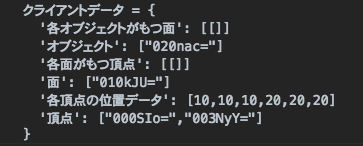
\includegraphics[scale=0.6]{images/init}
	 \caption{初期データ}
	 \label{init}
 \end{center}
\end{figure}
また, クライアントは4秒ごとに差分を計算しサーバからの返信が着き次第適用処理を行う. 最後のクライアントが実験を開始して5分10秒後に各クライアントのデータが一致しているか確かめた.
%%%%%%%%%%%%%%%%%%%%%%%%%%%%%%%%%%
%    実験結果
%%%%%%%%%%%%%%%%%%%%%%%%%%%%%%%%%%
\subsection{実験結果}
用意した全ての基本命令を処理した後のクライアント1の結果を図\ref{kekka1}に, クライアント2の結果を図\ref{kekka2}に,クライアント3の結果を図\ref{kekka3}に示す.
各図に示す通り, 各クライアントのデータは一致した.
\begin{figure}[]
 \begin{center}
	 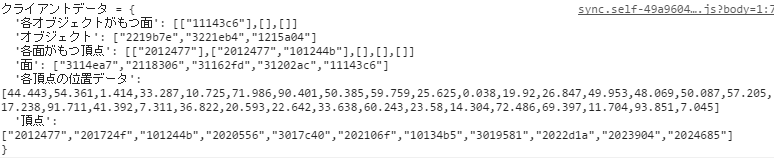
\includegraphics[scale=0.6]{images/kekka1}
	 \caption{クライアント1の結果}
	 \label{kekka1}
 \end{center}
\end{figure}
\begin{figure}[]
 \begin{center}
	 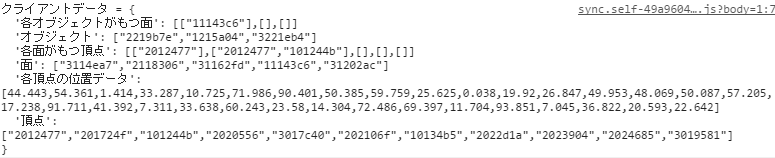
\includegraphics[scale=0.6]{images/kekka2}
	 \caption{クライアント2の結果}
	 \label{kekka2}
 \end{center}
\end{figure}
\begin{figure}[]
 \begin{center}
	 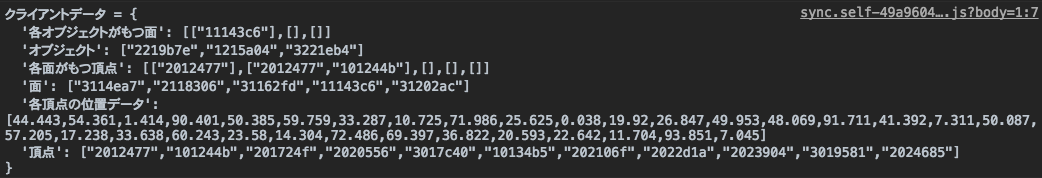
\includegraphics[scale=0.3]{images/kekka3}
	 \caption{クライアント3の結果}
	 \label{kekka3}
 \end{center}
\end{figure}
%%%%%%%%%%%%%%%%%%%%%%%%%%%%%%%%%%
%    考察
%%%%%%%%%%%%%%%%%%%%%%%%%%%%%%%%%%
\subsection{考察}
各クライアントのデータが一致したので,
本研究での提案手法による同期機構で3次元データは同期可能であった.
